\chapter{Baseline Architecture: ResNet-50 + LSTM}

To evaluate the architectural advantages of the hierarchical Swin Transformer and cross-attention language decoding, we compare it against the classical encoder--decoder paradigm established by Vinyals et al.~[1] and Pranay Kumar et al.~[9]: an ImageNet-pretrained convolutional network (CNN) paired with a recurrent Long Short-Term Memory (LSTM) decoder. Both models are trained, tuned, and evaluated on identical splits of the ROCOv2 benchmark.

\section{Architectural Pipeline}

Figure 4.1 contrasts the baseline topology with our proposed framework.

\begin{figure}[!htbp]
\centering
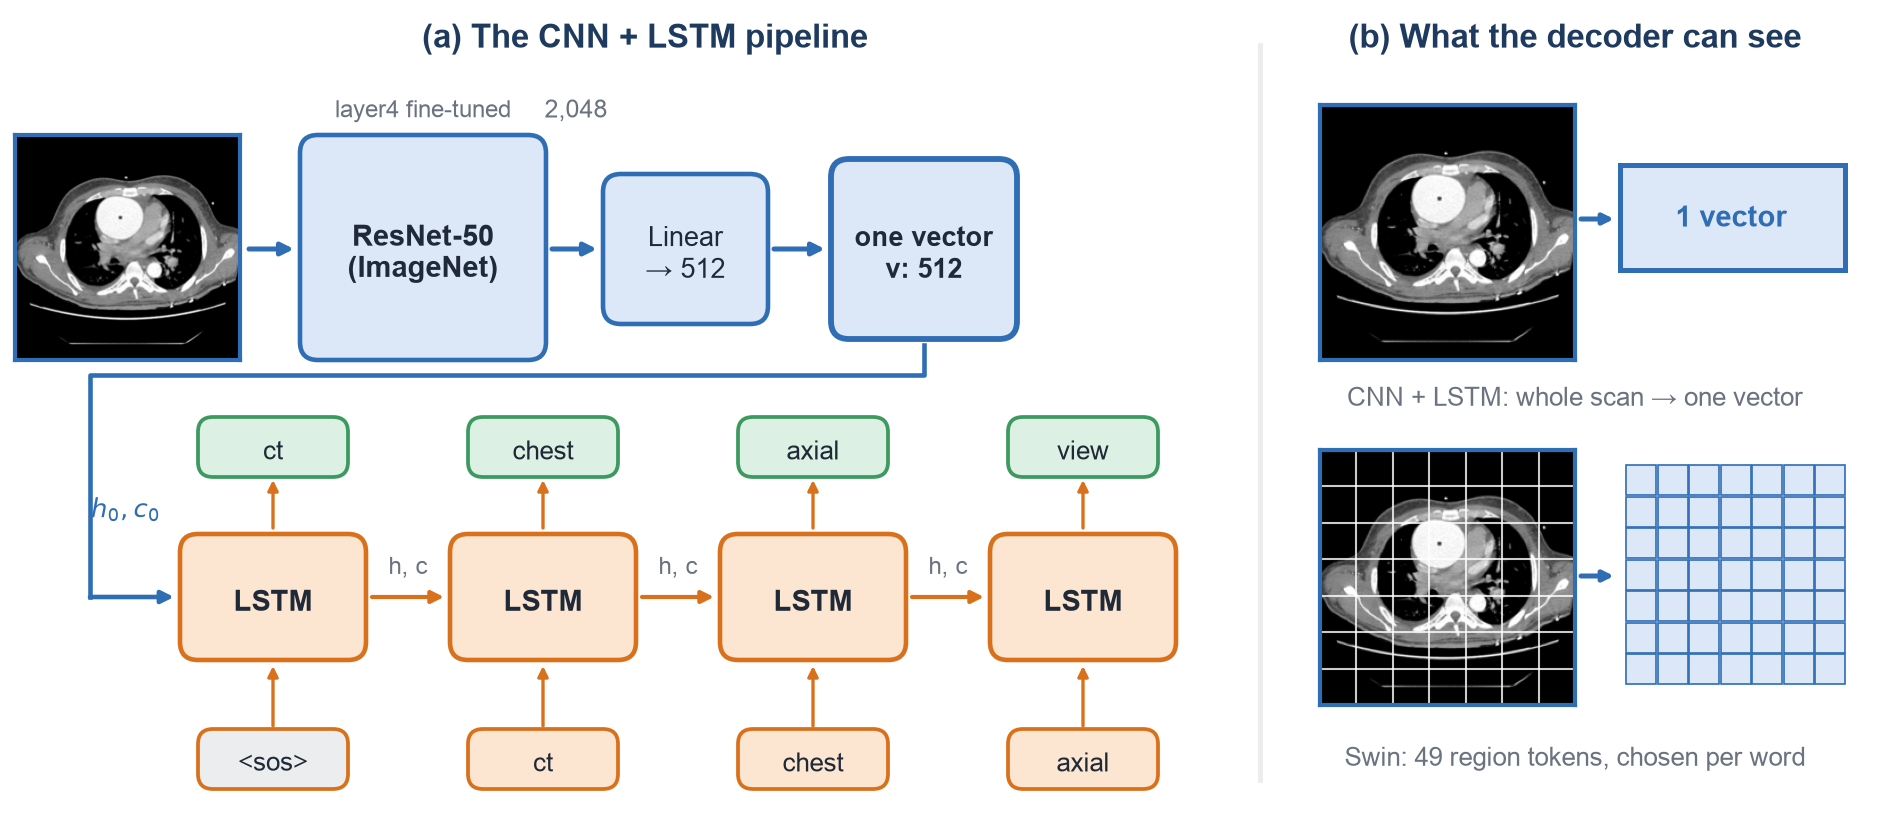
\includegraphics[width=0.95\linewidth,height=\textheight,keepaspectratio]{figures/fig4_1_cnn_lstm.png}
\caption{(a) The classical ResNet-50 + LSTM pipeline: visual features are collapsed into a single 512-dimensional vector that initializes the recurrent memory cells. (b) Architectural comparison: the LSTM relies on a static global vector, whereas the Swin Transformer provides dynamic cross-attention across 49 localized spatial memory tokens.}
\end{figure}

\begin{itemize}
\item \textbf{Visual Feature Extraction:} A ResNet-50 backbone pretrained on ImageNet-1K extracts visual representations. The final convolutional feature map ($7 \times 7 \times 2048$) is compressed via global average pooling into a single vector $v_{\text{raw}} \in \mathbb{R}^{2048}$, followed by a linear projection to $d_{\text{proj}} = 512$.
\item \textbf{Recurrent Decoder:} A 1-layer LSTM ($d_{\text{hidden}} = 512$, $d_{\text{embed}} = 512$) generates text word-by-word. The projected visual vector initializes the recurrent hidden state ($h_0$) and cell state ($c_0$).
\item \textbf{Two-Stage Training:} The ResNet-50 backbone is initially frozen for 2 epochs, after which its final residual block (\texttt{layer4}) is unfrozen for end-to-end fine-tuning with AdamW ($\text{lr} = 1.0 \times 10^{-4}$ for the head, $1.0 \times 10^{-5}$ for the backbone) across 16 epochs.
\end{itemize}

\section{Mathematical Formulation}

The global visual feature vector $v \in \mathbb{R}^{512}$ initializes the LSTM hidden state $h_0$ and cell state $c_0$:

\begin{equation}
v = W_p\, \mathrm{AvgPool}\left(\mathrm{ResNet}_{50}(I)\right) + b_p \in \mathbb{R}^{512}, \qquad h_0 = \tanh(W_h v), \quad c_0 = \tanh(W_c v) \tag{4.1}
\end{equation}

At each decoding step $t$, the LSTM updates its cell state $c_t$ and hidden state $h_t$ through gating operations:

\begin{equation}
\begin{pmatrix} f_t \\ i_t \\ o_t \\ g_t \end{pmatrix} = \begin{pmatrix} \sigma \\ \sigma \\ \sigma \\ \tanh \end{pmatrix} \left( W\, [e_t \,\|\, h_{t-1}] + b \right) \tag{4.2}
\end{equation}

\begin{equation}
c_t = f_t \odot c_{t-1} + i_t \odot g_t, \qquad h_t = o_t \odot \tanh(c_t) \tag{4.3}
\end{equation}

The output vocabulary distribution is projected via an affine transformation: $\ell_t = W_{\text{out}} h_t + b_{\text{out}} \in \mathbb{R}^{|V|}$.

\begin{takeawaybox}
\textbf{The Spatial Compression Bottleneck.}
In the CNN-LSTM design, the entire radiograph (including localized focal lesions, subtle opacities, and anatomical margins) is compressed into a single vector ($1 \times 512$) injected exclusively at $t=0$. The LSTM possesses no mechanism to re-examine spatial regions as text generation unfolds. Consequently, recurrent decoders frequently experience vanishing visual conditioning over long horizons, collapsing into the high-frequency language prior.
\end{takeawaybox}
